\pdfoutput=1
\pdfcompresslevel=9
\pdfinfo
{
    /Author (Aleksy Barcz)
    /Title (Implementation aspects of graph neural networks)
    /Keywords (Graph neural networks, classification, graph processing, recursive neural networks)
}
%\documentclass[a4paper,polish,onecolumn,oneside,floatssmall,11pt,titleauthor,wide,openright]{mwrep}
%\usepackage[scale={0.7,0.8},paper=a4paper,twoside]{geometry}
\documentclass[a4paper,onecolumn,oneside,12pt,wide,floatssmall]{mwrep} % 11pt w szablonie, 12pt dla TimesNewRoman
\usepackage{amsmath}
\usepackage{amsfonts}
\usepackage{amssymb}
\usepackage{amsthm}
\usepackage{bookman}
\usepackage{bm}		% bold math symbols

\usepackage{geometry}
\usepackage[utf8x]{inputenc}
\usepackage[T1]{fontenc}
% \usepackage{t1enc}
% \usepackage[pdftex, bookmarks]{hyperref}
%\usepackage[pdftex, bookmarks=false]{hyperref}
\usepackage[pdftex, bookmarks=true, colorlinks=true,linkcolor=black,urlcolor=blue,citecolor=black]{hyperref}
%\def\url#1{{ \tt #1}}
\usepackage{url} % linki url w bibliografii
\usepackage{alltt}
\usepackage{booktabs} % eleganckie tabelki
\usepackage{mathtools} % wyrównane macierze, wymaga texlive-latex3
\usepackage{bm} % pogrubione greckie litery

\usepackage{listings}

\usepackage{pslatex} %Times New Roman

% marginesy
\textwidth\paperwidth
\advance\textwidth -55mm
\oddsidemargin-0.9in
\advance\oddsidemargin 33mm
\evensidemargin-0.9in
\advance\evensidemargin 33mm
\topmargin -1in
\advance\topmargin 13mm
\setlength\textheight{48\baselineskip}
\addtolength\textheight{\topskip}
\marginparwidth15mm

\clubpenalty=10000 % to kara za sierotki
\widowpenalty=10000 % nie pozostawia wdów
\brokenpenalty=10000 % nie dzieli wyrazów pomiędzy stronami
\sloppy

\tolerance4500
\pretolerance250
\hfuzz=1.5pt
\hbadness1450

\linespread{1.3}	% interlinia 1.5 linii

% dotfill with smaller dots
\makeatletter
\newcommand \Dotfill {\leavevmode \cleaders \hb@xt@ .25em{\hss .\hss }\hfill \kern \z@}
\makeatother

% ŻYWA PAGINA
\renewcommand{\chaptermark}[1]{\markboth{\scshape\small\bfseries \
#1}{\small\bfseries \ #1}}
\renewcommand{\sectionmark}[1]{\markboth{\scshape\small\bfseries\thesection.\
#1}{\small\bfseries\thesection.\ #1}}
\newcommand{\headrulewidth}{0.5pt}
\newcommand{\footrulewidth}{0.pt}
\pagestyle{uheadings}

\usepackage[pdftex]{color,graphicx}
\usepackage[english]{babel}
\usepackage[usenames,dvipsnames]{xcolor} % kolory dla listingow kodu

\usepackage{parcolumns}	% two-column paragraphs
\usepackage{subfigure}
\usepackage{floatrow}
% Table float box with bottom caption, box width adjusted to content
\newfloatcommand{capbtabbox}{table}[][\FBwidth]


% \textheight232mm
% \setlength{\textwidth}{\textwidth}
% \setlength{\oddsidemargin}{\evensidemargin}
% \setlength{\evensidemargin}{0.3cm}
\usepackage[sort, compress]{cite}

%\usepackage{multibib}
%\newcites{bk,st,doc,web}{Książki i~artykuły,Standardy i~zalecenia,Dokumentacja produktów,Publikacje i~serwisy internetowe}

\theoremstyle{definition}
\newtheorem{defn}{Definition}[section]
\newtheorem{exmp}{Example}[section]

\theoremstyle{plain}% default
\newtheorem{thm}{Theorem}[section]
\newtheorem{lem}[thm]{Lemma}
\newtheorem{prop}[thm]{Hipothesis}
\newtheorem*{cor}{Conclusion}

\theoremstyle{remark}
\newtheorem*{rem}{Remark}
\newtheorem*{note}{Remark}
\newtheorem{case}{Case}

\definecolor{ListingBackground}{rgb}{1,1,1}

\begin{document}

% kody źródłowe wplatane w tekst
\lstdefinestyle{incode}
{
basicstyle={\footnotesize},
keywordstyle={\bf\footnotesize\color{black}},
commentstyle={\em\footnotesize\color{gray}},
numbers=left,
stepnumber=5,
firstnumber=1,
numberfirstline=true,
numberblanklines=true,
numberstyle={\sf\tiny},
numbersep=10pt,
tabsize=2,
xleftmargin=17pt,
framexleftmargin=3pt,
framexbottommargin=2pt,
framextopmargin=2pt,
framexrightmargin=0pt,
showstringspaces=true,
backgroundcolor={\color{ListingBackground}},
extendedchars=true,
% title=\lstname,
captionpos=b,
% abovecaptionskip=1pt,
% belowcaptionskip=1pt,
frame=tb,
framerule=0pt,
}

% kody źródłowe z podpisem
\lstdefinestyle{outcode}
{
basicstyle={\footnotesize},
keywordstyle={\bf\footnotesize\color{black}},
commentstyle={\em\footnotesize\color{gray}},
numbers=left,
stepnumber=5,
firstnumber=1,
numberfirstline=true,
numberblanklines=true,
numberstyle={\sf\tiny},
numbersep=10pt,
tabsize=2,
xleftmargin=17pt,
framexleftmargin=3pt,
framexbottommargin=2pt,
framextopmargin=2pt,
framexrightmargin=0pt,
showstringspaces=true,
backgroundcolor={\color{ListingBackground}},
extendedchars=true,
% title=\lstname,
captionpos=b,
% abovecaptionskip=1pt,
% belowcaptionskip=1pt,
frame=tb,
framerule=0.1pt,
}

\pagenumbering{roman}
\renewcommand{\baselinestretch}{1.0}
\raggedbottom
%
\begin{titlepage}
    % Strona tytułowa
    \vbox to\textheight{\hyphenpenalty=10000
    \begin{center}
	\begin{tabular}{p{107mm} p{9cm}}
	    \begin{minipage}{9cm}
	      \begin{center}
	      Politechnika Warszawska \\
	      Wydział Elektroniki i~Technik Informacyjnych \\
	      Instytut Informatyki
	      \end{center}
	    \end{minipage}
	    &
	    \begin{minipage}{8cm}
	    \begin{flushleft}
	      Rok akademicki 2012/2013
	    \vspace*{2.75\baselineskip}
	    \end{flushleft}
	    \end{minipage} \\
	\end{tabular}
	\vspace*{2.5\baselineskip}
	\begin{center}
		
\includegraphics[height=3.5cm,width=3.5cm]{img/PW_logo.png}
	\end{center}
	\vspace*{2.2\baselineskip}{\Large \MakeUppercase{Praca dyplomowa magisterska}\par}
	\vspace{2\baselineskip}{\large Aleksy Stanisław Barcz\par}
	\vspace*{2\baselineskip}{\LARGE Implementation aspects of graph neural networks\par}

	\vspace*{7\baselineskip}
	\hfill\mbox{}\par\vspace*{\baselineskip}\noindent
	\begin{tabular}[b]{@{}p{3cm}@{\ }l@{}}
	    {\large\hfill } & {\large }
	\end{tabular}
	\hfill
	\begin{tabular}[b]{c}
		Opiekun pracy: \\
		{mgr inż. Zbigniew Szymański}
	\end{tabular}\par
	\vspace*{5\baselineskip}
    \begin{tabular}{p{\textwidth}}
    \begin{flushleft}
	\begin{minipage}{7cm}
	Ocena: \Dotfill
	\par\vspace{2.5\baselineskip}
	\Dotfill
	\vspace{0.5\baselineskip}
	\par\noindent
	\centerline{Podpis Przewodniczącego}
	\centerline{Komisji Egzaminu Dyplomowego}\par
	\end{minipage}
    \end{flushleft}
    \end{tabular}
    \end{center}}

    % Życiorys
    \newpage\thispagestyle{empty}
    \begin{tabular}{p{4cm} p{20cm}}
    \begin{minipage}{4cm}
    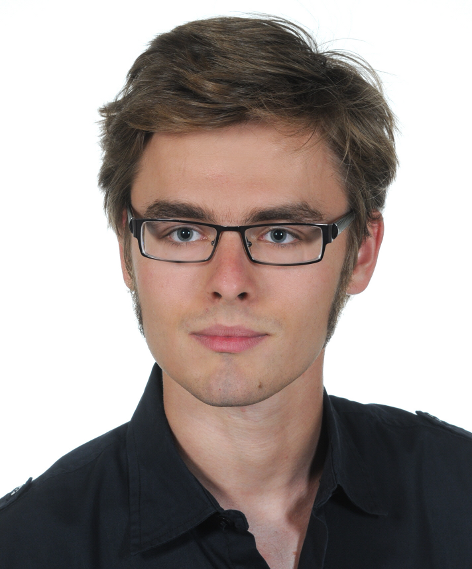
\includegraphics[height=4.8cm,width=4cm]{img/myphoto_cropped.png}
    \end{minipage}
    &
    \begin{minipage}{20cm}
    \begin{flushleft}
    \par\noindent\vspace{1\baselineskip}
    \begin{tabular}[h]{l l}
    {\normalsize Kierunek:} & Informatyka\\
    {\normalsize Specjalność:} & Inżynieria systemów informatycznych
    \end{tabular}
    \par\noindent\vspace{2\baselineskip}
    \begin{tabular}[h]{l r}
    {\normalsize Data urodzenia:} & {\normalsize 1988.01.28} \\
    {\normalsize Data rozpoczęcia studiów:} & {\normalsize 2012.02.20}
    \end{tabular}
    \par\noindent\vspace{2\baselineskip}
    \end{flushleft}
    \end{minipage}
    \end{tabular}
    \vspace*{1\baselineskip}
    \begin{center}
	{Życiorys}\par\bigskip
    \end{center}

    \noindent
	Ukończyłem XXVIII LO im. J.Kochanowskiego w Warszawie, w klasie o profilu matematyczno - informatycznym. Studia inżynierskie ukończyłem w lutym 2012 roku na kierunku Informatyka na Wydziale Elektroniki i Technik Informacyjnych Politechniki Warszawskiej. W trakcie studiów I i II stopnia brałem udział w wymianach studenckich programu Athens na Katholieke Universiteit Leuven \emph{(Fundamentals of artificial intelligence)} oraz w Télécom ParisTech \emph{(Emergence in complex systems)}.
    \par
    \vspace{2\baselineskip}
    \hfill\parbox{15em}{{\small\Dotfill}\\[-.3ex]
    \centerline{Podpis studenta}}\par
    \vspace{3\baselineskip}
 	{\noindent\MakeUppercase{Egzamin dyplomowy}} \par\bigskip\bigskip
    \par\noindent\vspace{1.5\baselineskip}
    Złożył egzamin dyplomowy w dniu \Dotfill 2013~r.
    \par\noindent\vspace{1.5\baselineskip}
    z wynikiem \Dotfill
    \par\noindent\vspace{1.5\baselineskip}
    Ogólny wynik studiów: \Dotfill
    \par\noindent\vspace{1.5\baselineskip}
    Dodatkowe wnioski i uwagi Komisji: \Dotfill
    \par\noindent\vspace{1.5\baselineskip}
    \Dotfill
    \par\noindent\vspace{1.5\baselineskip}
    \Dotfill

    % Streszczenie
    \newpage\thispagestyle{empty}
    \vspace*{2\baselineskip}
    \begin{center}
	{\large \MakeUppercase{Summary}}\par\bigskip
    \end{center}

    {\noindent
	This thesis describes the process of implementation of a Graph Neural Network, a classifier capable of classifying data represented as graphs. Parameters affecting the classifier efficiency and the learning process were identified and described. Implementation details affecting the classifier efficiency were described. Important similarities to other connectionist models used for graph processing were highlighted.
	}
    \vspace*{1\baselineskip}

    \noindent{Keywords}: {Graph neural networks, classification, graph processing, recursive neural networks}
    \par
    \vspace{4\baselineskip}

	\begin{center}
	\line(1,0){250}
	\end{center}

    \begin{center}
	{\large \MakeUppercase{ASPEKTY IMPLEMENTACYJNE GRAFOWYCH SIECI NEURONOWYCH}}\par\bigskip
    \end{center}
    {\noindent
	Praca stanowi raport z samodzielnej implementacji klasyfikatora typu Graph Neural Network (grafowa sieć neuronowa), pozwalającego na klasyfikację danych o strukturze grafowej. W ramach pracy zidentyfikowane zostały istotne dla klasyfikatora parametry, wpływające na przebieg procesu uczenia się klasyfikatora oraz na jakość uzyskanych wyników. Opisane zostały szczegóły implementacyjne klasyfikatora istotne dla jego działania. Klasyfikator został przedstawiony w kontekście podobnych rozwiązań w celu ukazania ścisłych powiązań między istniejącymi modelami przetwarzania danych o strukturze grafowej, opartymi na sieciach neuronowych.
	}
	
    \vspace*{1\baselineskip}

    \noindent{Słowa kluczowe}: {Grafowe sieci neuronowe, klasyfikacja, przetwarzanie grafów, rekursywne sieci neuronowe}

\end{titlepage}

% ex: set tabstop=4 shiftwidth=4 softtabstop=4 noexpandtab fileformat=unix filetype=tex spelllang=pl,en spell:

%
\begin{titlepage}
    % Strona tytułowa
    \vbox to\textheight{\hyphenpenalty=10000
    \begin{center}
	\begin{tabular}{p{107mm} p{9cm}}
	    \begin{minipage}{9cm}
	      \begin{center}
	      Politechnika Warszawska \\
	      Wydział Elektroniki i~Technik Informacyjnych \\
	      Instytut Informatyki
	      \end{center}
	    \end{minipage}
	    &
	    \begin{minipage}{8cm}
	    \begin{flushleft}
	      Rok akademicki 2012/2013
	    \vspace*{2.75\baselineskip}
	    \end{flushleft}
	    \end{minipage} \\
	\end{tabular}
	\vspace*{2.5\baselineskip}
	\begin{center}
		
\includegraphics[height=3.5cm,width=3.5cm]{img/PW_logo.png}
	\end{center}
	\vspace*{2.2\baselineskip}{\Large \MakeUppercase{Praca dyplomowa magisterska}\par}
	\vspace{2\baselineskip}{\large Aleksy Stanisław Barcz\par}
	\vspace*{2\baselineskip}{\LARGE Implementation aspects of graph neural networks\par}

	\vspace*{7\baselineskip}
	\hfill\mbox{}\par\vspace*{\baselineskip}\noindent
	\begin{tabular}[b]{@{}p{3cm}@{\ }l@{}}
	    {\large\hfill } & {\large }
	\end{tabular}
	\hfill
	\begin{tabular}[b]{c}
		Opiekun pracy: \\
		{mgr inż. Zbigniew Szymański}
	\end{tabular}\par
    \end{center}}

\end{titlepage}

% ex: set tabstop=4 shiftwidth=4 softtabstop=4 noexpandtab fileformat=unix filetype=tex spelllang=pl,en spell:


%\tableofcontents
% \addcontentsline{toc}{chapter}{{Przedmowa1}{vii}}{vii}

%\setlength{\baselineskip}{7mm}
\newpage
\pagenumbering{arabic}
\setcounter{page}{1}

\appendix
%
\chapter{Penalty calculation equations}


\chapter{Using the software\label{chapter:using}}
\noindent The GNN classifier was implemented in GNU Octave 3.6.2 and tested on a x86\_64 PC. The most important functions are:
\begin{itemize}
	\item loadgraph - loads a single graph from .csv files
	\item loadset - loads a set of graphs sharing the same filename prefix
	\item mergegraphs - merge a cellarray of graphs to a single graph
	\item initgnn - initialize a new GNN
	\item traingnn - train GNN using a training graph
	\item classifygnn - classify given graph with a trained GNN
	\item evaluate - evaluate the classification results
	\item crossvalidate - perform cross-validation using an untrained GNN and a set of graphs
\end{itemize}
\noindent Help and usage information for each function can be displayed by typing \emph{help <function\_name>} in the Octave command line.\\



\begin{lstlisting}[style=outcode, language=Matlab, caption=Sample usage session]
g6 = loadset('../data/g6s3n/g6s3', 10);
gm = mergegraphs(g6);
gnn = initgnn(gm, 5, [5 5], 'tansig');
trainedGnn = traingnn(gnn, gm, 20);
outputs = classifygnn(trainedGnn, gm);
stats = evaluate(outputs, gm.expectedOutput);
\end{lstlisting}

\noindent All subgraph matching datasets were created using the \emph{buildgraphs.py} script. Each graph can be viewed as a pdf file by using the \emph{drawgraph.py} script. Each graph is stored as three .csv files, containing node labels, edge labels and expected outputs. A sample graph \emph{'test'} is presented below. Nodes yielding output 2 were marked as black.

\begin{figure}
\begin{floatrow}
\ffigbox[\FBwidth]{	% use the image width
	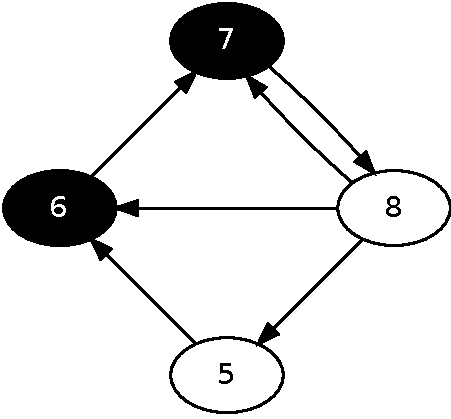
\includegraphics[scale=0.55]{img/test}
}{
\caption{Sample graph}
}
\capbtabbox{
	\begin{tabular}{lll}
	\toprule
	test\_nodes.csv & test\_output.csv & test\_edges.csv \\
	\midrule
	5	&	1	&	1,2,0\\
	6	&	2	&	2,3,0\\
	7	&	2	&	3,4,0\\
	8	&	1	&	4,1,0\\
		&		&	4,2,0\\
		&		&	4,3,0\\
	\bottomrule
	\end{tabular}
}{
\caption{Sample graph data}%
}
\end{floatrow}
\end{figure}


%\listoftables
%\listoffigures
% \lstlistoflistings

%\nocite{*}
%\bibliographystyle{plplain}
\bibliographystyle{ieeetr}
%\bibliographystylebk{plplain}
%\bibliographystylest{plplain}
%\bibliographystyledoc{plplain}
% \bibliographystyleweb{plplain}
%\bibliographybk{BIB/books}
%\bibliographyst{BIB/books}
%\bibliographydoc{BIB/books}
% \bibliographyweb{BIB/books}


\end{document}

% ex: set tabstop=4 shiftwidth=4 softtabstop=4 noexpandtab fileformat=unix filetype=tex spelllang=pl,en spell:

